\documentclass[11pt]{article}

\usepackage[T1]{fontenc}
\usepackage{lmodern}
\usepackage{amsmath,amssymb}
\usepackage{graphicx}
\usepackage{tikz}
\usepackage{hyperref}
\usepackage[margin=1in]{geometry}

\title{Intrinsic NCOS: Definition and Program}
\date{}

\begin{document}
\maketitle

\section{Goal}
Define whether NCOS is intrinsically well defined as a perturbative open string theory, independent of presentation details. In this note we focus on the Type II \emph{superstring} NCOS, since only that version is generally believed to be quantum-mechanically consistent.

\section{Candidate Intrinsic Definition}
Take NCOS to be the collection of open-string amplitudes obtained by the scaling limit
\[
E \to 1^{-}, \qquad \alpha' \to 0,
\]
with $\alpha'_{\mathrm{eff}}$ and $G_o$ fixed, applied to parent D-brane string amplitudes:
\[
\mathcal{A}^{\mathrm{NCOS}}_{g,n}
=
\lim_{E\to 1^{-},\,\alpha'\to 0}
\mathcal{A}^{\mathrm{parent}}_{g,n}(E,\alpha').
\]
NCOS is intrinsically well defined perturbatively if this set is closed and consistent on its own.

\section{BCFT of Superstring NCOS (Already in the Limit)}
\label{sec:bcft}
The NCOS BCFT is defined directly in terms of renormalized open-string data
\[
\alpha'_e,\qquad G_o,\qquad \theta^{01}=2\pi\alpha'_e,
\]
and renormalized boundary fields $(\mathbb X^M,\Psi^M)$ whose correlators are finite. We choose the open-string frame where the surviving open metric is canonical.

\subsection*{Renormalized Boundary Algebra}
For longitudinal directions $\alpha,\beta=0,1$,
\[
\langle \mathbb X^\alpha(\tau)\mathbb X^\beta(0)\rangle
=-2\alpha'_e\eta^{\alpha\beta}\ln|\tau|
+\frac{i}{2}\theta^{\alpha\beta}\,\mathrm{sgn}(\tau),
\qquad
\theta^{01}=2\pi\alpha'_e.
\]
For transverse directions $i,j=2,\dots,9$ (after renormalization of fields),
\[
\langle \mathbb X^i(\tau)\mathbb X^j(0)\rangle
=-2\alpha'_e\delta^{ij}\ln|\tau|.
\]
Boundary fermions obey
\[
\langle \Psi^M(\tau)\Psi^N(0)\rangle
=\frac{G_{\mathrm{op}}^{MN}}{\tau},
\]
with $G_{\mathrm{op}}^{MN}=\eta^{MN}$ in this frame. Zero modes satisfy
\[
[\mathbb x^0,\mathbb x^1]=i\theta^{01}=i\,2\pi\alpha'_e.
\]

\subsection*{Worldsheet Superconformal Structure}
In terms of renormalized fields, the boundary stress tensor and supercurrent are
\[
T=-\frac{1}{2\alpha'_e}G^{\mathrm{op}}_{MN}:\partial\mathbb X^M\partial\mathbb X^N:
-\frac12 G^{\mathrm{op}}_{MN}:\Psi^M\partial\Psi^N:,
\]
\[
T_F=i\sqrt{\frac{2}{\alpha'_e}}\,G^{\mathrm{op}}_{MN}\Psi^M\partial\mathbb X^N.
\]
This is the NSR superstring BCFT underlying perturbative NCOS amplitudes.

\subsection*{Renormalized Operators and OPE}
Boundary exponentials satisfy
\[
:e^{ik\cdot\mathbb X(\tau)}::e^{iq\cdot\mathbb X(0)}:
\sim
|\tau|^{2\alpha'_e G_{\mathrm{op}}^{MN}k_M q_N}
e^{-\frac{i}{2}k\wedge q\,\mathrm{sgn}(\tau)}
:e^{i(k+q)\cdot\mathbb X(0)}:,
\]
where $k\wedge q\equiv k_M\theta^{MN}q_N$. The logarithmic piece fixes scaling dimensions; the antisymmetric piece gives Moyal phases.

Representative NS vertex operator:
\[
V_{\mathrm{NS}}^{(-1)}=\zeta_M\Psi^M e^{-\phi}e^{ik\cdot\mathbb X}.
\]
BRST gives
\[
L_0=\alpha'_e G_{\mathrm{op}}^{MN}k_Mk_N+N-a=0,
\qquad a_{\mathrm{NS}}=\frac12,\quad a_{\mathrm{R}}=0.
\]
In components (with mostly-plus signature),
\[
\alpha'_e\!\left(-k_0^2+k_1^2+k_\perp^2\right)+N-a=0,
\qquad
k_\perp^2\equiv \sum_{i=2}^{9}k_i^2.
\]
Only in the special $1+1$ subsector with $k_i=0$ does this reduce to
\[
k_+k_-=\frac{N-a}{\alpha'_e}.
\]

\subsection*{Perturbative Amplitudes}
At fixed genus $g$, amplitudes are computed from this BCFT with coupling weight $G_o^{\,2g-2+n}$. Ordered boundary insertions differ by the phase
\[
\exp\!\left(\frac{i}{2}\sum_{a<b}k_a\wedge k_b\,\mathrm{sgn}(\tau_a-\tau_b)\right),
\]
while the remaining kernel contains the full superstring contractions, including transverse $\mathbb X^i,\Psi^i$ excitations and polarizations:
\[
\mathcal A^{\mathrm{ord}}_{g,n}
=
e^{\frac{i}{2}\sum_{a<b}k_a\wedge k_b\,\mathrm{sgn}(\tau_a-\tau_b)}
\,
\mathcal K^{\mathrm{ord}}_{g,n}\!\left(\alpha'_e;\{k_i,\zeta_i,\text{oscillators}\}\right).
\]
The physical amplitude then sums/integrates over orderings and moduli. Thus NCOS does not truncate away the transverse sector; simplifications from $k_i=0$ apply only to that restricted kinematic subsector.

\subsection*{Why Superstring Only}
The bosonic analog is not considered a reliable quantum theory (tachyon instability and additional electric-background pathologies). The Type II superstring version with GSO projection is the one believed to define a consistent perturbative NCOS sector.

\section{Intrinsic BCFT Mechanism for Simplified Dynamics}
\label{sec:intrinsic_mechanism}
The simplification is structural, not a claim that all amplitudes are easy. For an ordered boundary configuration $\sigma$, the genus-zero integrand can be written schematically as
\[
\mathcal I_\sigma
=
\mathcal K_{\perp,\sigma}\,
\prod_{a<b}|\tau_{ab}|^{2\alpha'_e k_a\!\cdot\! k_b}\,
\exp\!\left(\frac{i}{2}\sum_{a<b}k_a\wedge k_b\,\mathrm{sgn}_\sigma(\tau_{ab})\right),
\]
where $\mathcal K_{\perp,\sigma}$ contains the full transverse/oscillator RNS contractions. Thus transverse dynamics is fully retained.

For open strings on a D1, $k_{ai}=0$ (Dirichlet directions), so all momentum dependence in the explicit Koba--Nielsen/phase factor is longitudinal $(0,1)$ data. The NCOS-specific input is the critical relation
\[
\theta^{01}=2\pi\alpha'_e.
\]
At this value, and with one external massless open-string state integrated first, the longitudinal part becomes a total derivative in the insertion coordinate:
\[
\mathcal I_\sigma(\tau_r)=\partial_{\tau_r}\mathcal F_\sigma(\tau_r).
\]
Equivalently: logarithmic monodromy from $|\tau_{ab}|^{2\alpha'_e k_a\cdot k_b}$ and ordering monodromy from the Moyal phase are locked at the same scale. This ``critical monodromy matching'' is what fails away from NCOS.

Therefore the full amplitude (sum over orderings) obeys
\[
\sum_\sigma\int d\tau_r\,\mathcal I_\sigma
=
\sum_\sigma\int d\tau_r\,\partial_{\tau_r}\mathcal F_\sigma
=0
\]
for amplitudes with at least one external massless open-string leg (tree level). The result is a block-triangular dynamical structure:
\begin{enumerate}
\item a decoupled massless $U(1)$ sector, and
\item an interacting massive open-string tower.
\end{enumerate}
This is the intrinsic BCFT origin of ``simpler NCOS dynamics'': strong selection rules from critical braiding, while the remaining massive transverse kernel is still stringy and nontrivial.

\section{Competing Mechanisms and How to Test Them}
\label{sec:competing_mechanisms}
The section above states one working mechanism. Below are six concrete possibilities for \emph{why} NCOS dynamics simplifies, formulated as falsifiable hypotheses.

\subsection*{1. Critical Braiding/Monodromy Matching}
\textbf{Idea.} The equality $\theta^{01}=2\pi\alpha'_e$ aligns phase monodromy with logarithmic monodromy.  
\textbf{Why it simplifies.} Ordering sums acquire linear dependencies; amplitudes with at least one massless leg cancel after summing permutations.  
\textbf{What to prove.} For fixed dynamical kernel $\mathcal K_{\perp,\sigma}$, show that the phase matrix over orderings has a null vector in the massless-leg sector:
\[
\sum_\sigma c_\sigma\,e^{i\Phi_\sigma}=0.
\]
\textbf{Failure mode.} If generic higher-point examples (with full oscillator structure) violate this null-vector condition, this mechanism is incomplete.

\subsection*{2. BRST/Cohomological Total-Derivative Mechanism}
\textbf{Idea.} In the NCOS BCFT, an integrated massless vertex is BRST-exact modulo a boundary derivative:
\[
V_{\mathrm{massless,int}}=\{Q,\Lambda\}+\partial_\tau \Omega.
\]
\textbf{Why it simplifies.} Moduli integrals localize to boundaries, and boundary pieces cancel across orderings due to NCOS phases.  
\textbf{What to prove.} Construct $\Lambda,\Omega$ explicitly in the renormalized NSR theory and show cancellation with full transverse kernel included.  
\textbf{Failure mode.} If branch-cut/boundary terms survive and do not cancel, decoupling is only partial.

\subsection*{3. Braided-Category/Transparent-Sector Mechanism}
\textbf{Idea.} Boundary operators form a braided algebra with braiding
\[
c_{ab}=e^{-\,\frac{i}{2}k_a\wedge k_b}.
\]
The massless $U(1)$ sector may be transparent (or effectively transparent after quotienting null states).  
\textbf{Why it simplifies.} The S-matrix becomes block-triangular: transparent sector decouples from interacting massive sector.  
\textbf{What to prove.} Construct the physical braided category after BRST quotient and identify whether massless operators lie in its center (exactly or effectively).  
\textbf{Failure mode.} Nontrivial monodromy with physical massive operators persists after quotient, invalidating transparency.

\subsection*{4. Zero-Mode Superselection Mechanism}
\textbf{Idea.} The Weyl algebra
\[
[\mathbb x^0,\mathbb x^1]=i\,2\pi\alpha'_e
\]
induces superselection labels (dipole/endpoint data) that constrain allowed transitions.  
\textbf{Why it simplifies.} Many channels are forbidden kinematically by sector mismatch, not by accidental cancellation.  
\textbf{What to prove.} Identify the conserved algebraic charge(s) at asymptotic boundaries and show that amplitudes mixing massless and interacting sectors violate the charge selection rule.  
\textbf{Failure mode.} If no conserved label survives BRST and asymptotic-state construction, this explanation collapses.

\subsection*{5. Moduli-Space Localization Mechanism}
\textbf{Idea.} In NCOS kinematics the relevant form on boundary-insertion moduli space becomes exact:
\[
\omega_n=d\beta_n
\]
for classes of external states (notably with a massless leg).  
\textbf{Why it simplifies.} Amplitudes reduce to boundary strata, where permutation/orientation structure enforces cancellations.  
\textbf{What to prove.} Write the full ordered integrand as a differential form on configuration space $\mathcal C_n(\mathbb R)$ and verify exactness plus boundary cancellation.  
\textbf{Failure mode.} Non-exact residues remain in interior moduli, giving nonzero contributions.

\subsection*{6. Emergent 1+1 Integrability of the Interacting Massive Sector}
\textbf{Idea.} After massless-sector decoupling, the remaining massive NCOS sector may exhibit factorized scattering (or a near-integrable deformation).  
\textbf{Why it simplifies.} Dynamics is then controlled by two-body data, bootstrap constraints, and possible CDD structure rather than generic string multiparticle complexity.  
\textbf{What to test.} Compute explicit $2\to2$ and $2\to n$ amplitudes in low levels; check particle production, Yang--Baxter consistency, and factorization of higher-point poles.  
\textbf{Failure mode.} Robust non-factorizing multiparticle production at generic kinematics rules this out.

\subsection*{Current Best Synthesis}
The strongest near-term route is likely a combination of (1)+(2)+(5): critical braiding sets the phase structure, BRST/cohomology turns one insertion into a derivative, and moduli-space geometry converts this into explicit ordering cancellations. Mechanisms (3) and (4) may provide a deeper algebraic interpretation; (6) is a high-risk/high-payoff endpoint.

\section{What BCFT Gives (and What It Does Not)}
The BCFT data in a near-critical electric background gives an intrinsic \emph{perturbative} definition:
\begin{enumerate}
\item on-shell vertex operators and correlators,
\item genus-by-genus amplitudes as an expansion in $G_o$,
\item the perturbative open-string spectrum around one background.
\end{enumerate}
By itself, this does \emph{not} yet provide a complete finite-coupling definition.

\section{Closure and Consistency Criteria}
\begin{enumerate}
\item \textbf{BRST/no-ghost consistency:}
Physical state space is well defined and gauge redundancies decouple.
\item \textbf{Open-string factorization:}
Residues of poles factorize into lower-point NCOS amplitudes.
\item \textbf{Perturbative unitarity:}
Optical-theorem/cutting relations hold within NCOS asymptotic states.
\item \textbf{Sector closure:}
No finite-energy leakage to additional asymptotic sectors in the chosen background.
\item \textbf{Genus stability of the limit:}
The scaling limit exists uniformly enough order-by-order in $G_o$.
\end{enumerate}

\section{Immediate Background Caveat}
\begin{enumerate}
\item \textbf{Noncompact spatial direction:}
Evidence supports a closed perturbative open sector at finite energy.
\item \textbf{Compact spatial direction:}
Wound closed strings can enter at finite energy; the pure-open sector is then not closed unless asymptotic states are enlarged.
\end{enumerate}

\section{Cylinder Diagram in Type II Superstring: No Closed-String Pole}
\label{sec:cylinder_superstring}
The relevant test is the \emph{nonplanar four-point annulus} with two open-string insertions on each boundary. This is the setup used in the classic NCOS/NCFT one-loop analyses (Minwalla--Seiberg--Van Raamsdonk; Bassetto \emph{et al.}).

\subsection*{Correct Kinematic Setup: 2+2 Boundary Insertions}
Label the external states so that $(k_1,k_2)$ sit on one boundary and $(k_3,k_4)$ on the other. The momentum exchanged between boundaries is
\[
K^\mu \equiv k_1^\mu+k_2^\mu = -(k_3^\mu+k_4^\mu).
\]
The nonplanar annulus is the piece that probes closed-channel singularities; the planar piece does not carry this inter-boundary transfer.

\begin{figure}[t]
\centering
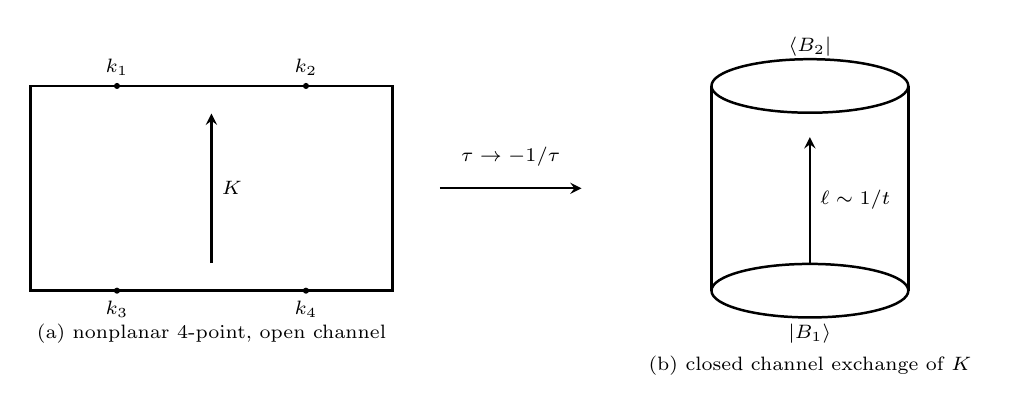
\begin{tikzpicture}[line width=0.9pt,>=stealth]
% (a) open-channel strip with 2+2 insertion pattern
\draw (0,0) rectangle (4.6,2.6);
\fill (1.1,2.6) circle (1.1pt);
\fill (3.5,2.6) circle (1.1pt);
\fill (1.1,0.0) circle (1.1pt);
\fill (3.5,0.0) circle (1.1pt);
\node[above] at (1.1,2.6) {\scriptsize $k_1$};
\node[above] at (3.5,2.6) {\scriptsize $k_2$};
\node[below] at (1.1,0.0) {\scriptsize $k_3$};
\node[below] at (3.5,0.0) {\scriptsize $k_4$};
\draw[->,thick] (2.3,0.35) -- (2.3,2.25);
\node[right] at (2.3,1.3) {\scriptsize $K$};
\node at (2.3,-0.55) {\scriptsize (a) nonplanar 4-point, open channel};

% modular arrow
\draw[->,thick] (5.2,1.3) -- (7.0,1.3);
\node at (6.1,1.7) {\scriptsize $\tau\to-1/\tau$};

% (b) closed-channel cylinder
\begin{scope}[xshift=7.8cm]
\draw (2.1,0.0) ellipse (1.25 and 0.34);
\draw (2.1,2.6) ellipse (1.25 and 0.34);
\draw (0.85,0.0) -- (0.85,2.6);
\draw (3.35,0.0) -- (3.35,2.6);
\draw[->,thick] (2.1,0.35) -- (2.1,1.95);
\node[right] at (2.1,1.15) {\scriptsize $\ell\sim1/t$};
\node at (2.1,3.1) {\scriptsize $\langle B_2|$};
\node at (2.1,-0.55) {\scriptsize $|B_1\rangle$};
\node at (2.1,-0.95) {\scriptsize (b) closed channel exchange of $K$};
\end{scope}
\end{tikzpicture}
\caption{Worldsheet duality for the nonplanar annulus 4-point test: two open insertions on each boundary and momentum transfer $K$ across the cylinder.}
\label{fig:annulus_worldsheet_duality}
\end{figure}

\subsection*{Superstring Input}
In this 4-point nonplanar setup, the closed-channel singularity condition is written in terms of
\[
K\circ K \equiv -K_\mu(\theta G\theta)^{\mu\nu}K_\nu,
\]
and one finds branch points at
\[
s\ge \frac{4n}{\alpha'}+\frac{1}{4\pi^2\alpha'^2}K\circ K,\qquad n=0,1,\dots
\]
for the Type II superstring. In a pure electric background ($\theta_{01}\equiv\theta_E$),
\[
K\circ K=\theta_E^2(s+K_T^2),\qquad
s_n(1-\widetilde E^2)=\widetilde E^2K_T^2+\frac{4n}{\alpha'}.
\]
The bosonic analog has an additional tachyonic sector; Type II GSO projection removes that instability. In NCOS variables, the effective threshold piece can be written as
\[
\Delta_{N_{\rm cl}}(s)\sim
\frac{p_\perp^2}{1-\widetilde E^2}
\,+\,\frac{4N_{\rm cl}}{\alpha'_e(1-\widetilde E^2)}
\,-\,s.
\]
So superstring consistency removes tachyonic poles already before taking the NCOS limit.

\subsection*{Explicit 2+2 Singular Piece (Analytic)}
For the Type II nonplanar 2+2 annulus, the superstring analysis of hep-th/0311120 gives (after required permutation symmetrization) a decomposition
\[
\mathcal A^{\rm np}_{2+2}
=\sum_{n\ge 0} f_{2n}(s_{\rm CL},d,|Y|)\,\alpha^S_{2n}(\text{kinematics},\theta),
\]
with odd levels removed by symmetrization. The closed-channel kernel is
\[
f_n \propto
\left(\frac{2\pi m\alpha'}{\,n-\alpha' s_{\rm CL}/4\,}\right)^{d/2-4}
K_{d/2-4}\!\left(4\pi\alpha' m\sqrt{n-\alpha' s_{\rm CL}/4}\right),
\]
so the analytic structure is controlled by the square root
\[
\sqrt{n-\frac{\alpha' s_{\rm CL}}{4}}.
\]
Therefore singularities arise at branch points (cuts), not simple poles, with threshold condition
\[
s\ge \frac{4n}{\alpha'}+\frac{1}{4\pi^2\alpha'^2}K\circ K,
\qquad n=0,1,\dots
\]
which is exactly the superstring branch condition quoted above.

Equivalent singular-part reduction (suppressing smooth polarization/theta-function prefactors):
\[
\mathcal A^{\rm np}_{2+2}(s)\propto
\sum_{n\ge 0}\int_0^\infty d\ell\;\ell^{-1/2}
\exp\!\big[-\ell\,(M_n^2-s-i0)\big],
\]
with
\[
M_n^2=\frac{4n}{\alpha'}+\frac{1}{4\pi^2\alpha'^2}K\circ K
\;=\;
\frac{\widetilde E^2K_T^2+4n/\alpha'}{1-\widetilde E^2}.
\]
The $\ell$-integral is explicit:
\[
\int_0^\infty d\ell\;\ell^{-1/2}e^{-\ell\Lambda}
=\Gamma\!\left(\frac12\right)\Lambda^{-1/2},
\]
so
\[
\mathcal A^{\rm np}_{2+2}(s)\propto
(M_n^2-s-i0)^{-1/2}.
\]
Hence the singularity is a branch point (cut), not a simple pole.
In electric variables ($\theta_{01}=\theta_E$), this is equivalently
\[
s_n\!\left(1-\frac{\theta_E^2}{4\pi^2\alpha'^2}\right)
=
\frac{\theta_E^2}{4\pi^2\alpha'^2}K_T^2+\frac{4n}{\alpha'},
\]
and with $\widetilde E=\theta_E/(2\pi\alpha')$:
\[
s_n(1-\widetilde E^2)=\widetilde E^2K_T^2+\frac{4n}{\alpha'},
\]
again matching the analytic formulas in hep-th/0311120. This is the key no-pole statement; numerics are only optional cross-checks.

\subsection*{Theta-Function Expansion in the 2+2 Nonplanar Integrand}
To make the analytic mechanism explicit, start from the superstring 2+2 nonplanar integrand (same notation as hep-th/0311120):
\[
\mathcal A_S(1,2)\sim
\int_0^1\frac{dq}{q}\,q^{\frac14 K g^{-1}K}\,(\log q)^{d/2-5}e^{Y^2/\log q}
\int d\nu_1 d\nu_2 d\nu_3\;\mathcal I(q,\nu).
\]
Using Jacobi product forms, one can write
\[
P_{\rm e}(\nu,q)\equiv\prod_{m\ge1}(1-2q^{2m}\cos2\pi\nu+q^{4m}),
\]
\[
P_{\rm o}(\nu,q)\equiv\prod_{m\ge1}(1-2q^{2m-1}\cos2\pi\nu+q^{4m-2}),
\]
so the integrand is a product of factors of the form
\[
[\sin(\pi\nu)\,P_{\rm e}(\nu,q)]^{-s/2},
\qquad
[P_{\rm o}(\nu,q)]^{-t/2},
\qquad
[P_{\rm o}(\nu,q)]^{-u/2},
\]
times Moyal phases.

For small $q$, writing $c\equiv \cos(2\pi\nu)$:
\[
P_{\rm e}(\nu,q)=1-2c\,q^2+(1-2c)\,q^4+(4c^2-2c)\,q^6+O(q^8),
\]
\[
P_{\rm o}(\nu,q)=1-2c\,q+q^2-2c\,q^3+4c^2q^4-4c\,q^5+(4c^2+1)q^6+O(q^7).
\]
These coefficients are obtained directly from the infinite products and checked against the Jacobi-theta identities with machine precision in \texttt{scratch/annulus\_q\_expansion\_check.py}.

hence
\[
\mathcal I(q,\nu)=\sum_{r\ge0}q^r\,\mathcal I_r(\nu;s,t,u,\theta).
\]
Therefore
\[
\mathcal A_S(1,2)=\sum_{r\ge0}\alpha_r^S(s,t,u,\theta)
\int_0^1 dq\;q^{-1+r-\frac14 s_{\rm CL}}(\log q)^{d/2-5}e^{Y^2/\log q},
\]
with $s_{\rm CL}=s-\frac{1}{4\pi^2\alpha'^2}K\circ K$.

Now impose the physical symmetrization in the $(1,2)$ channel:
\[
\mathcal A_S^{\rm sym}=\mathcal A_S(1,2)+\mathcal A_S(2,1).
\]
As shown in the superstring analysis (their Appendix B logic), odd-$r$ terms are antisymmetric and drop out:
\[
\alpha_{2n+1}^S=0,\qquad
\mathcal A_S^{\rm sym}=\sum_{n\ge0}\alpha_{2n}^S\,f_{2n}(s_{\rm CL},d,|Y|).
\]
So the ``pole cancellation'' statement is analytic: first, unphysical odd-level terms are removed by symmetrization; second, the surviving $f_{2n}$ have square-root/Bessel branch structure, yielding cuts rather than isolated closed-string poles in the noncompact NCOS kinematics.

\subsection*{Why There Is No Closed-String Pole}
For noncompact $x^1$, $q_1$ is continuous. Therefore each level contributes
\[
\int_{-\infty}^{\infty}\frac{dq_1}{q_1^2+\Delta-i0}
\;=\;
\pi(\Delta-i0)^{-1/2},
\]
which has a square-root branch point at $\Delta=0$ and a cut for $\Delta<0$, not an isolated pole. Thus the closed channel is branch-cut type in noncompact kinematics.

\begin{figure}[t]
\centering
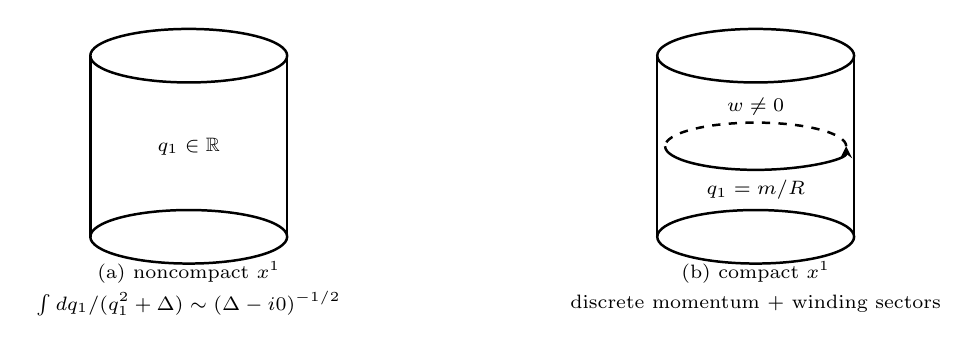
\begin{tikzpicture}[line width=0.9pt,>=stealth]
\begin{scope}
\draw (2.1,0.0) ellipse (1.25 and 0.34);
\draw (2.1,2.3) ellipse (1.25 and 0.34);
\draw (0.85,0.0) -- (0.85,2.3);
\draw (3.35,0.0) -- (3.35,2.3);
\node at (2.1,1.15) {\scriptsize $q_1\in\mathbb R$};
\node at (2.1,-0.45) {\scriptsize (a) noncompact $x^1$};
\node at (2.1,-0.85) {\scriptsize $\int dq_1/(q_1^2+\Delta)\sim(\Delta-i0)^{-1/2}$};
\end{scope}

\begin{scope}[xshift=7.2cm]
\draw (2.1,0.0) ellipse (1.25 and 0.34);
\draw (2.1,2.3) ellipse (1.25 and 0.34);
\draw (0.85,0.0) -- (0.85,2.3);
\draw (3.35,0.0) -- (3.35,2.3);
\draw[->] (0.95,1.15) arc[start angle=180,end angle=360,x radius=1.15,y radius=0.30];
\draw[dashed] (3.25,1.15) arc[start angle=0,end angle=180,x radius=1.15,y radius=0.30];
\node at (2.1,1.65) {\scriptsize $w\neq 0$};
\node at (2.1,0.60) {\scriptsize $q_1=m/R$};
\node at (2.1,-0.45) {\scriptsize (b) compact $x^1$};
\node at (2.1,-0.85) {\scriptsize discrete momentum + winding sectors};
\end{scope}
\end{tikzpicture}
\caption{Worldsheet kinematics of the closed channel: noncompact longitudinal direction gives continuum momentum and threshold cut; compactification allows discrete momentum and winding sectors.}
\label{fig:compact_vs_noncompact_worldsheet}
\end{figure}

\subsection*{NCOS Scaling of the Branch Point}
Equivalent annulus branch-point kinematics can be written as
\[
s_n(1-\widetilde E^2)=\widetilde E^2K_T^2+\frac{4n}{\alpha'},
\]
with $\widetilde E=\theta_E/(2\pi\alpha')$. In the NCOS scaling
\[
\alpha'=\alpha'_e(1-\widetilde E^2),\qquad \widetilde E\to1^-,
\]
this becomes
\[
s_n
\sim
\frac{\widetilde E^2K_T^2}{1-\widetilde E^2}
\,+\,\frac{4n}{\alpha'_e(1-\widetilde E^2)^2}
\to\infty
\]
for any $n>0$ or $K_T\neq0$. Hence at fixed finite external energy, closed-string singularities are pushed out of reach.

So in the Type II superstring NCOS sector (noncompact $x^1$):
\begin{enumerate}
\item there is no tachyonic closed-string pole (GSO),
\item there is no isolated closed-string pole even kinematically (continuous $q_1$ gives cuts, not poles),
\item and the relevant closed-channel branch points are driven to infinite $s$ in the NCOS limit for finite-energy scattering.
\end{enumerate}
The exceptional $n=0$, $K_T=0$ corner is a threshold branch point at $s=0$ (forward/zero-transfer limit), not a finite-$s$ pole.

The compact case is different: discrete momentum/winding sectors can reintroduce finite-energy closed-string asymptotic states, consistent with the caveat above.

\section{Missing Nonperturbative Recipe (Open-String Viewpoint)}
\label{sec:missing_recipe}
To claim an intrinsic nonperturbative NCOS definition from the open-string side, one needs:
\begin{enumerate}
\item \textbf{Finite-coupling object:}
A definition of $Z_{\mathrm{NCOS}}(G_o,\alpha'_{\mathrm{eff}})$, not only an asymptotic series in $G_o$.
\item \textbf{Nonperturbative sectors:}
A principled inclusion of contributions of order $e^{-c/G_o}$ (which saddles exist, and with what measure).
\item \textbf{All-genus channel closure:}
A proof that moduli-space degenerations are closed within the proposed asymptotic state space, or a precise enlargement if not.
\item \textbf{Off-shell gauge-complete definition:}
An OSFT-level functional integral with a well-defined contour and gauge treatment in the time-like noncommutative setting.
\item \textbf{Nonperturbative unitarity/completeness:}
A statement that the resulting Hilbert space and amplitudes satisfy exact unitarity beyond term-by-term perturbation theory.
\end{enumerate}
Without these ingredients, BCFT provides a strong perturbative sector, but not yet a standalone nonperturbative completion.

\section{Working Hypothesis}
\begin{enumerate}
\item Intrinsic perturbative NCOS exists as a consistent S-matrix sector in noncompact $1+1$.
\item A standalone nonperturbative definition in purely open-string variables is not yet established because the recipe in Section~\ref{sec:missing_recipe} is incomplete.
\item The cleanest candidate completion is likely through the dual SYM flux-sector definition.
\end{enumerate}

\section{Program (Physics-First)}
\begin{enumerate}
\item \textbf{Formalize axioms:}
State exactly which closure criteria are required for an intrinsic perturbative definition.
\item \textbf{Build an evidence map:}
For each criterion, record strongest support and known loopholes.
\item \textbf{Stress-test closure:}
Identify corners where extra sectors can re-enter.
\item \textbf{Formulate the missing recipe explicitly:}
For each item in Section~\ref{sec:missing_recipe}, write a candidate construction and its obstruction.
\item \textbf{Decide the target claim:}
Either
\begin{itemize}
\item intrinsic perturbative sector exists under assumptions $X$, or
\item intrinsic nonperturbative definition requires enlargement beyond open strings alone.
\end{itemize}
\end{enumerate}

\section{Current Claim Template}
In noncompact $1+1$ kinematics, NCOS defines a perturbatively consistent open-string sector closed under factorization and unitarity at finite external energy, while compactification reintroduces wound closed-string channels and invalidates strict pure-open closure.

\section{Open Questions}
\begin{enumerate}
\item Can one construct a finite-$G_o$ object whose weak-coupling expansion reproduces NCOS BCFT amplitudes?
\item What are the relevant nonperturbative saddles, and how are they weighted in an open-string-only formulation?
\item Can one prove all-genus closure/factorization without importing parent closed-string channels?
\item Is there an OSFT contour/gauge prescription that is mathematically controlled in the time-like noncommutative regime?
\item In compact backgrounds, what is the minimal asymptotic-state enlargement needed for exact unitarity?
\end{enumerate}

\section{Claude Commentary}

\subsection*{Logical Relationships Among the Six Mechanisms}

The six mechanisms in Section~\ref{sec:competing_mechanisms} are not logically independent. They decompose into three tiers:

\medskip\noindent
\textbf{Tier 1: Three faces of one phenomenon (1 + 2 + 5).}
Critical braiding (1), the BRST/cohomological total-derivative (2), and moduli-space localization (5) are different mathematical framings of the same physical content. The chain of logic is:
\begin{itemize}
\item[(2)] In the NCOS BCFT, the integrated massless vertex operator, when inserted into a correlator with other boundary operators, yields an integrand that is a total $\tau$-derivative. This is the worldsheet \emph{origin}: it follows from the specific structure of the massless vertex in the renormalized theory, where BRST invariance combined with the critical noncommutativity $\theta^{01}=2\pi\alpha'_e$ conspires to make the longitudinal dependence exact.

\item[(1)] That total-derivative property implies that all orderings share the same boundary-evaluated kernel (up to phases), and the Moyal phases then provide the null vector in the ordering sum. This is the \emph{combinatorial consequence} of (2).

\item[(5)] Packaging the same information geometrically: the integrand, viewed as a differential form on the configuration space $\mathcal{C}_n(\mathbb{R})$ of ordered boundary insertions, is exact. The amplitude reduces to boundary strata, and the orientation/phase structure on those strata enforces the cancellation. This is the \emph{geometric packaging}.
\end{itemize}
A complete proof of massless decoupling at tree level would naturally use all three languages: (2) supplies the why, (1) supplies the how, and (5) supplies the clean mathematical statement. They should not be tested separately---rather, one should construct the proof in the language of (5), with (2) providing the key input and (1) emerging as an output.

\medskip\noindent
\textbf{Tier 2: Algebraic abstraction (3 + 4).}
The braided-category mechanism (3) is a higher-level reformulation: if the massless operators lie in the M\"uger center of the braided monoidal category of physical boundary operators (after BRST quotient), then decoupling is an algebraic theorem rather than a case-by-case cancellation.

The zero-mode superselection mechanism (4) would, if correct, be the strongest of all: it would make decoupling \emph{kinematic} (forbidden by a conserved charge) rather than \emph{dynamic} (vanishing by cancellation). However, there are reasons for caution. The Stone--von Neumann theorem guarantees a unique irreducible representation of the Weyl algebra for fixed $\theta$, so there is no discrete label arising from inequivalent representations. The ``dipole length'' $\Delta x^1 = \theta^{01}k_0$ is energy-dependent, not a fixed quantum number, and in the time-like noncommutative setting the physical interpretation of any superselection structure is less transparent than in the spatial case. One would need to identify a genuinely conserved grading of the NCOS Hilbert space (perhaps from the decomposition under the Weyl algebra tensored with the oscillator algebra) that separates the massless from the massive sector. If such a grading exists, it would provide the deepest explanation, but its construction is a nontrivial step that goes beyond what the current note establishes.

\medskip\noindent
\textbf{Tier 3: A separate question (6).}
Emergent integrability of the massive sector is \emph{not} an alternative explanation for the simplification discussed in mechanisms (1)--(5). It is a logically downstream question: \emph{after} the massless sector has decoupled (by whatever mechanism), does the remaining interacting massive tower have additional structure? Integrability and massless decoupling address different phenomena and should be investigated independently. That said, demonstrating (or falsifying) integrability would have major implications for the nonperturbative completion question in Section~\ref{sec:missing_recipe}.

\subsection*{The Boundary-Term Question}

The central claim of Section~\ref{sec:intrinsic_mechanism} is
\[
\sum_\sigma\int d\tau_r\,\partial_{\tau_r}\mathcal F_\sigma = 0.
\]
For this to hold, $\mathcal F_\sigma$ must either vanish at the boundary of the moduli-space integration region or cancel between orderings. At tree level, fixing three points by $SL(2,\mathbb{R})$ and integrating the remaining $n-3$ insertion points, the boundaries of the $\tau_r$ integration are the collision limits $\tau_r\to\tau_s$ (OPE channels). These are precisely where the Koba--Nielsen factor $|\tau_{rs}|^{2\alpha'_e k_r\cdot k_s}$ produces singularities or zeros.

The cleanest version of the argument (as elaborated in the companion note, lines 293--308 of the main draft) is contour-based: if the massless vertex is holomorphic in the insertion variable (after choosing branch cuts), the integration contour can be deformed off the boundary without crossing singularities. The different orderings then correspond to the same contour integral with different phase assignments, and the phases sum to zero (roots-of-unity cancellation). In this formulation, boundary terms do not arise because the contour is closed.

This contour-pulling argument is clean for the simplest cases (e.g., one massless leg among 3--4 external states, where the toy model with third roots of unity applies directly). The nontrivial extension is to:
\begin{enumerate}
\item[(a)] higher multiplicity ($n > 4$) with full transverse/oscillator structure in $\mathcal K_{\perp,\sigma}$,
\item[(b)] cases where multiple massless legs are present (which should give stronger vanishing but requires checking that the multi-dimensional contour deformation is unobstructed),
\item[(c)] cases where the transverse kernel $\mathcal K_\perp$ introduces additional branch points that could obstruct holomorphy.
\end{enumerate}
Item (c) is the real concern: the transverse contractions involve factors like $|\tau_{ab}|^{2\alpha'_e k_{a,\perp}\cdot k_{b,\perp}}$, but on the D1 all $k_\perp=0$, so these factors are unity. The remaining transverse structure comes from fermion/oscillator contractions, which are polynomial in $\tau_{ab}^{-1}$---hence meromorphic, not branch-cut-producing. This is reassuring: on the D1, the contour-deformation argument should close without transverse obstructions. But this reasoning should be made explicit in the proof.

\subsection*{Higher-Genus Extension}

The total-derivative/monodromy-matching argument is stated for tree level (genus zero). Extending it requires addressing two separate issues:

\medskip\noindent
\textbf{One-loop massless decoupling.} At genus one (annulus), the worldsheet has an additional modular parameter $q$ (or equivalently the cylinder length $t$). The boundary insertion moduli are now positions on the two boundary circles. The question is: does the integrand, with a massless vertex on one boundary, still become a total derivative in the insertion variable? If so, the same phase-cancellation argument would apply ordering-by-ordering, and massless decoupling would extend to one loop. The main draft (lines 360--418) establishes that \emph{closed-string} thresholds go to infinity in the NCOS limit---but this is about heavy-state decoupling, not about massless open-string decoupling at one loop. These are logically distinct: the first says ``no new light states from closed strings''; the second says ``the massless open-string $U(1)$ remains free at one loop.'' Both would need to hold for full perturbative consistency.

\medskip\noindent
\textbf{Closed-string channels in the annulus.}
Even if unwound bulk closed strings decouple (thresholds $\to\infty$), the annulus amplitude in ordinary open string theory always admits a closed-string channel interpretation via modular transformation ($q\to\tilde q = e^{-2\pi^2/\ln q}$). In the NCOS limit, the relevant question is whether the modular transformation commutes with the limit. The analysis in the main draft shows that the closed-channel branch points are pushed to infinite $s$ as $\widetilde E\to 1$, which is the correct statement for sector closure at one loop. But one should verify that the \emph{amplitude} itself (not just its singularity structure) is well-defined in the limit: it could happen that the amplitude diverges mildly (e.g., logarithmically in $1-\widetilde E^2$) even though singularities decouple. Such divergences, if present, would need to be absorbed into NCOS coupling renormalization.

\subsection*{Underuse of Supersymmetry}

Neither note makes heavy use of the $(8,8)$ supersymmetry of the D1-brane worldvolume theory. This is a significant omission. The superalgebra in 1+1 dimensions with 16 supercharges is extremely constraining:
\begin{itemize}
\item The massive open-string states organize into long multiplets of the $(8,8)$ algebra. The massless vector (the decoupling $U(1)$) sits in a short/BPS multiplet. Supersymmetric Ward identities relate amplitudes involving different members of the same multiplet, which could provide an independent route to the decoupling statement: if one mixed massless-massive amplitude vanishes (by the mechanisms above), supersymmetry forces all related amplitudes to vanish as well.
\item Non-renormalization theorems may protect the tree-level decoupling to all loops, reducing the higher-genus extension discussed above to a finite check.
\item The massive spectrum should admit a classification by $(8,8)$ representations. This representation-theoretic structure could make the braided-category mechanism (3) tractable: one would analyze braiding representation-by-representation rather than state-by-state.
\end{itemize}
A targeted computation: derive the $(8,8)$ Ward identities for a mixed amplitude $\langle V_{\mathrm{massless}} V_{\mathrm{massive}} V_{\mathrm{massive}} V_{\mathrm{massive}}\rangle$ at tree level, and check whether supersymmetry alone (without invoking monodromy matching) forces it to vanish. If it does, the decoupling is protected by supersymmetry, which is a stronger statement than monodromy cancellation.

\subsection*{The Integrability Question in Depth}

Mechanism (6) deserves a more detailed assessment. The massive NCOS sector in 1+1 noncompact dimensions has the ingredients that make integrability plausible:
\begin{itemize}
\item It is a 1+1d theory of massive particles.
\item The spectrum is an infinite Regge tower $m_N^2 = (N-a)/\alpha'_e$, $N=1,2,\ldots$.
\item The parent theory (Type IIB on D1) has maximal supersymmetry.
\item The noncommutativity introduces a natural deformation parameter.
\end{itemize}
However, there are reasons for skepticism:
\begin{itemize}
\item In standard open string theory in flat space, the S-matrix is \emph{not} integrable: there is genuine particle production (e.g., $2\to 4$ processes). The NCOS limit modifies the amplitudes by Moyal phases, but does not obviously eliminate all production channels.
\item Integrable 1+1d models with infinite particle towers exist (e.g., strings in $\mathrm{AdS}_3\times S^3$, the principal chiral model at the WZW point), but they typically arise from an underlying infinite-dimensional symmetry algebra (affine Lie algebra, Yangian, etc.). One would need to identify such a symmetry in the NCOS context.
\item The simplest test---absence of particle production in $2\to 2$ scattering of the lightest massive state---can be checked by explicit computation. If there is nonzero $2\to 3$ production at tree level in the massive sector, integrability is ruled out. If it vanishes, one should check Yang--Baxter for the $2\to 2$ S-matrix and look for a CDD structure (zeros/poles at specific rapidities).
\end{itemize}
The connection to integrability also has a nonperturbative angle: if the massive NCOS sector is integrable, the exact S-matrix can be written down via the bootstrap, and the finite-coupling completion (item 1 of Section~\ref{sec:missing_recipe}) becomes an S-matrix bootstrap problem rather than a path-integral problem. This would be a radical simplification of the nonperturbative question.

\subsection*{What ``Intrinsic'' Really Means and the SYM Completion}

The note's working hypothesis (Section~9) states that the nonperturbative completion comes through the dual SYM flux sector. This raises a conceptual point about the goal of the note. If the nonperturbative \emph{definition} of NCOS is a sector of $\mathcal{N}=(8,8)$ $U(N)$ SYM (in the $k=1$ electric flux superselection sector, at the energy scale $E\sim g_{\mathrm{YM}}/N$), then:
\begin{itemize}
\item At finite coupling, NCOS ``is'' a sector of a gauge theory, and its intrinsicness is inherited from the gauge theory.
\item The open-string language is the weak-coupling ($G_o\to 0$, i.e., $N\to\infty$) description of this gauge theory sector.
\item The perturbative BCFT data are the asymptotic expansion of gauge-theory observables in $1/N$.
\end{itemize}
In this picture, the question ``is NCOS intrinsically well-defined?'' becomes ``is the $k=1$ electric flux sector of 2d $\mathcal{N}=(8,8)$ $U(N)$ SYM a well-defined subsector of the gauge theory?'' The answer is yes if:
\begin{enumerate}
\item[(i)] Electric flux is exactly superselected (it is: it is a topological quantum number in 2d gauge theory on $\mathbb{R}^{1,1}$, being the holonomy at spatial infinity).
\item[(ii)] The Hilbert space within this sector is well-defined nonperturbatively.
\item[(iii)] The S-matrix restricted to this sector satisfies unitarity.
\end{enumerate}
Conditions (i) and (ii) hold for the gauge theory by standard arguments. Condition (iii) is subtler: it requires that scattering within the flux sector does not leak probability into other sectors or into the continuum. In the noncompact case, this should hold because flux is conserved.

This suggests that the \emph{existence} of intrinsic nonperturbative NCOS is not in doubt if one accepts the SYM definition---the question is whether one can \emph{derive} the open-string perturbation theory from it, and whether there is an independent open-string-variable formulation. The note's program (Section~11) is then more precisely: establish that the BCFT perturbative data match the $1/N$ expansion of flux-sector gauge theory observables, and determine what additional input (beyond the BCFT) is needed to reconstruct the exact answer.

\subsection*{Suggested Computations}

Ordered roughly by difficulty and payoff:
\begin{enumerate}
\item \textbf{4-point massless amplitude at tree level, explicit.} Verify the roots-of-unity cancellation with the full NSR vertex operators (not just the toy model). This is the minimal check of the monodromy-matching mechanism, and it should be straightforward given existing technology.

\item \textbf{Mixed 4-point: one massless + three massive (lowest level).} Verify vanishing. This tests decoupling beyond the pure-massless sector and exercises the contour-deformation argument with nontrivial oscillator structure in $\mathcal K_\perp$.

\item \textbf{5-point with one massless leg.} Verify vanishing. This is the first nontrivial higher-point test---at 5 points, there are more orderings and the phase structure is richer (fifth roots of unity for certain orderings, but the actual phases depend on the momenta, not just the number of legs). A failure here would be significant.

\item \textbf{$2\to 3$ massive production at tree level.} If this is nonzero, integrability (mechanism 6) is ruled out. If it vanishes, compute the $2\to 2$ massive S-matrix and check the Yang--Baxter equation.

\item \textbf{$(8,8)$ Ward identities for mixed amplitudes.} Determine whether supersymmetry alone forces massless-massive mixing amplitudes to vanish. If so, the decoupling is protected beyond tree level.

\item \textbf{One-loop annulus with one massless boundary insertion.} Check whether the total-derivative structure survives at genus one. This is computationally intensive but would establish massless decoupling at the next order.

\item \textbf{Construct the braided category of physical boundary operators.} Classify the BRST-physical boundary operators as objects in a braided monoidal category, compute their braiding, and determine whether the massless sector is in the M\"uger center.

\end{enumerate}

\subsection*{Time-Like Noncommutativity and the Unitarity Question}

A persistent worry about NCOS is that it involves time-like noncommutativity ($\theta^{01}\neq 0$), which in field theory leads to unitarity violations. The Seiberg--Susskind--Toumbas argument (hep-th/0005015) shows that noncommutative field theory with time-space $\theta$ produces acausal behavior: the effective interaction is nonlocal in time, and the Hamiltonian is not manifestly bounded below. Concretely, in NCFT with $\theta^{0i}\neq 0$, the Moyal star product generates interactions that mix positive- and negative-frequency modes, leading to pair creation from the vacuum and violations of the optical theorem at loop level.

NCOS is supposed to evade this problem because it is a \emph{string} theory, not a field theory. The infinite tower of massive open-string states provides UV softening that tames the acausal behavior. The argument is:
\begin{enumerate}
\item[(a)] At energies $E\ll 1/\sqrt{\alpha'_e}$, the theory looks like a noncommutative field theory with $\theta^{01}=2\pi\alpha'_e$, and unitarity violations appear.
\item[(b)] But these violations are artifacts of truncating the string to its lowest mode. The full string amplitude, including the entire massive tower, is UV-soft (exponential Regge falloff) and restores unitarity.
\item[(c)] The critical relation $\theta^{01}=2\pi\alpha'_e$ ensures that the noncommutativity scale and the string scale are locked: one can never probe the noncommutative regime without also exciting massive string modes.
\end{enumerate}
Point (c) is the key: in NCOS, there is no regime where noncommutative field theory is valid without stringy corrections, because $\theta\sim\alpha'_e$ identically. This is unlike the Seiberg--Witten field theory limit, where $\theta$ is held fixed while $\alpha'\to 0$, producing a genuine NCFT.

This has implications for the program. Any attempt to formulate NCOS dynamics in a truncated language (e.g., keeping only the massless mode, or using open string field theory truncated to level $N$) will encounter the time-like unitarity problem. The full infinite tower is essential. This is a strong constraint on mechanism (4) (zero-mode superselection): if the decoupling explanation involves only the zero-mode Weyl algebra, one must ask whether it is consistent with the need for the full tower to maintain unitarity. A purely zero-mode argument that works mode-by-mode might miss the essential stringy restoration.

It also constrains the OSFT approach (item 4 of Section~\ref{sec:missing_recipe}): any open string field theory formulation must be ``string-complete'' (not level-truncated) to preserve unitarity. Level-truncation studies of NCOS would necessarily exhibit time-like unitarity pathologies at finite truncation, recovering good behavior only in the $N\to\infty$ limit of levels. This is a practical obstruction to numerical OSFT approaches.

\subsection*{Deformation Away from Criticality}

A useful diagnostic is to consider the one-parameter family of theories with
\[
\theta^{01} = 2\pi\alpha'_e(1+\epsilon),
\]
where $\epsilon=0$ is the NCOS point and $\epsilon\neq 0$ is a deformation. In the parent D-brane language, this corresponds to $\widetilde E = 1-\delta$ with $\delta$ not tuned to produce the critical relation. The monodromy matching fails at order $\epsilon$:
\begin{itemize}
\item The logarithmic monodromy is controlled by $\alpha'_e$: $|\tau_{ab}|^{2\alpha'_e k_a\cdot k_b}$.
\item The phase monodromy is controlled by $\theta$: $\exp(-\frac{i}{2}k_a\wedge k_b)$ with $k_a\wedge k_b = k_{a,\alpha}\theta^{\alpha\beta}k_{b,\beta}$.
\item At the NCOS point these are locked; away from it, the contour-deformation argument fails because the integrand acquires a discontinuity of order $\epsilon$ when the contour crosses a branch cut.
\end{itemize}
This means the massless-massive coupling amplitude should scale as
\[
\mathcal{A}_{\mathrm{mixed}} \sim \epsilon \cdot (\text{kinematic factor}),
\]
vanishing linearly as $\epsilon\to 0$. Verifying this scaling in an explicit computation (say, the 4-point mixed amplitude near the NCOS point) would be a clean test of the mechanism: it confirms that the decoupling is specifically tied to $\theta = 2\pi\alpha'_e$ and not to some other structural feature of the theory.

The deformation also has a physical interpretation in the SYM dual. From the main draft, $\widetilde E = N\widetilde g_B/\sqrt{1+N^2\widetilde g_B^2}$, and the NCOS point is $\widetilde E\to 1$. Deforming $\epsilon\neq 0$ corresponds to finite $N$ corrections in the gauge theory. The massless-massive coupling of order $\epsilon\sim 1/N^2$ is then a $1/N^2$ effect in the gauge theory, which is the expected order for non-planar corrections that mix the $U(1)$ center with the $SU(N)$ factor.

\subsection*{Higher-Dimensional NCOS}

The decoupling mechanism in Section~\ref{sec:intrinsic_mechanism} is stated for the D1-brane, where all transverse momenta vanish ($k_i=0$ for Dirichlet directions $i=2,\ldots,9$). This is the cleanest setting because the Koba--Nielsen factor depends only on longitudinal momenta, and the critical relation $\theta^{01}=2\pi\alpha'_e$ controls the entire phase/monodromy structure.

For NCOS on a D$p$-brane with $p>1$, the electric field is still in the $(0,1)$ direction, but the brane extends in $p-1$ additional Neumann directions with coordinates $x^a$, $a=2,\ldots,p$. Open-string momenta $k_a$ along these directions are nonzero. The Koba--Nielsen factor then includes terms
\[
\prod_{a<b}|\tau_{ab}|^{2\alpha'_e(k_{a,\mathrm{long}}\cdot k_{b,\mathrm{long}} + k_{a,\parallel}\cdot k_{b,\parallel})},
\]
where $k_\parallel$ is the along-the-brane momentum outside the electric plane. The phase factor still involves only the $(0,1)$ noncommutativity (since $\theta^{ab}=0$ for $a,b\geq 2$ in a pure electric background). Now the contour-deformation argument is modified: the integrand is no longer holomorphic in the massless insertion variable because the $k_\parallel$-dependent Koba--Nielsen factors introduce branch cuts in $\tau_r$ that are not controlled by $\theta$.

Concretely, for a massless vertex with $k_{r,+}k_{r,-}=0$ but $k_{r,\parallel}\neq 0$, the factor $|\tau_{rs}|^{2\alpha'_e k_{r,\parallel}\cdot k_{s,\parallel}}$ is a genuine branch cut that obstructs the contour deformation. The result is that massless decoupling \emph{fails} for generic momenta in higher-dimensional NCOS---the $U(1)$ sector couples to the massive tower when along-the-brane momentum exchange is nonzero.

This failure has a clean physical interpretation: in $p+1>2$ dimensions, the massless photon has transverse polarizations and genuine long-range interactions. There is no reason for it to decouple. The decoupling in 1+1 is special because a $U(1)$ gauge field in 1+1 dimensions has no propagating degrees of freedom (no transverse polarizations). The NCOS critical braiding mechanism is the stringy incarnation of this familiar field-theory fact.

The conclusion for the program: \textbf{intrinsic NCOS with full massless decoupling is specific to the D1-brane (1+1 dimensions).} Higher-dimensional versions are consistent string theories but lack the block-triangular structure, and their ``simplicity'' is of a different character (noncommutative deformation of open string amplitudes without a decoupled sector).

\subsection*{The Compact Case: Wound Strings and Asymptotic-State Enlargement}

The robust point is that compactification changes the asymptotic Hilbert space. For noncompact $x$, unwound bulk closed strings decouple at finite external energy. For compact
\[
x\sim x+2\pi R,
\]
the winding sectors are physical, and in the NCOS limit one obtains finite-energy \emph{wound} closed strings with nonrelativistic dispersion (for $w>0$) of the form
\[
p_0=\frac{wR}{2\alpha'_e}+\frac{\alpha'_e k_\perp^2}{2wR}+\frac{N_L+N_R}{wR},
\]
rather than the naive relativistic estimate from the pre-limit mass formula. This is the standard wound-string/NRCS result in near-critical electric backgrounds (Gomis--Ooguri, hep-th/0009181).

So the safe statement is not a delicate scaling of $R/\sqrt{\alpha'}$, but:
\begin{itemize}
\item \textbf{Noncompact limit} ($R\to\infty$ at fixed finite scattering energy): wound states are kinematically heavy and effectively absent.
\item \textbf{Compact NCOS} (finite $R$): wound closed strings with $w>0$ are finite-energy states and must be included for exact unitarity/factorization.
\item \textbf{T-dual/SYM channel}: these winding sectors map to momentum/flux sectors in the dual description, consistent with the NCOS/SYM dictionary.
\end{itemize}
From the SYM perspective, the relevant charged sectors are automatic in the full gauge-theory Hilbert space. The issue appears only if one tries to define a strictly pure-open-string compact theory. Thus ``intrinsic NCOS'' in compact space is intrinsic to an enlarged
\[
\mathcal H_{\rm asym}=\mathcal H_{\rm open}\oplus\mathcal H_{\rm wound},
\]
not to $\mathcal H_{\rm open}$ alone.

\subsection*{NCOS in the Web of Decoupling Limits}

NCOS does not exist in isolation. It sits in a web of interrelated decoupling limits of string/M-theory, and the ``intrinsicness'' question arises in each:

\medskip\noindent
\textbf{NCSYM (Noncommutative Super-Yang--Mills).}
The Seiberg--Witten field theory limit: $\alpha'\to 0$ with $G,\theta$ fixed. This produces a noncommutative gauge theory, which is manifestly intrinsic (it is defined by a Lagrangian). But in the electric ($\theta^{0i}\neq 0$) case, it suffers from the unitarity problems discussed above, which are cured only by embedding into the full NCOS. In the magnetic case ($\theta^{ij}\neq 0$, $i,j$ spatial), NCSYM is unitary and well-defined. The comparison is instructive: magnetic NCSYM is an intrinsic QFT; electric NCSYM requires stringy completion (NCOS).

\medskip\noindent
\textbf{OM theory (Open Membrane theory).}
Arises from M-theory membranes in a near-critical 3-form $C$-field background. It is the M-theory uplift of NCOS: upon dimensional reduction on the M-theory circle, OM theory reduces to NCOS. The intrinsicness question for OM theory is even harder because there is no perturbative formulation of membranes to serve as a starting point. If NCOS admits an intrinsic perturbative definition, the M-theory uplift to OM theory would need a nonperturbative definition from the start.

\medskip\noindent
\textbf{Little String Theory (LST).}
Arises from the decoupling limit of NS5-branes. Like NCOS, it is a non-gravitational theory with a string scale but no adjustable Planck scale. LST has a Hagedorn density of states and is believed to be a well-defined theory, but no Lagrangian formulation exists. The intrinsicness question for LST has been studied via its holographic dual (the linear dilaton background), and the consensus is that LST is intrinsically defined by its holographic dual. The analogy to NCOS is close: in both cases, the perturbative string description is available but the nonperturbative completion is best accessed through a dual description.

\medskip\noindent
\textbf{DLCQ of M-theory / Matrix theory.}
The BFSS matrix model defines the DLCQ of M-theory as a specific quantum mechanics. This is an example where a decoupling limit \emph{does} produce an intrinsically defined theory (the matrix model Lagrangian). The NCOS/SYM duality is a dimensional uplift of the same structure: NCOS in 1+1d is dual to 2d SYM in the flux sector, analogous to how DLCQ M-theory is dual to matrix quantum mechanics. The flux-sector restriction is the analogue of the DLCQ light-cone momentum quantization.

The pattern across all these limits is consistent: perturbative string/membrane descriptions exist and are useful, but nonperturbative definitions come from dual gauge-theoretic formulations. NCOS fits this pattern exactly. The intrinsic perturbative BCFT data are analogous to the perturbative string amplitudes in little string theory or the loop expansion in matrix theory; the nonperturbative completion comes from the SYM flux sector.

\subsection*{Nonperturbative Saddles and D-Brane Effects}

Item 2 of Section~\ref{sec:missing_recipe} asks about nonperturbative contributions of order $e^{-c/G_o}$. In the NCOS context, with $G_o^2 = 1/N$, these are effects of order $e^{-c\sqrt{N}}$ (or $e^{-cN}$ depending on the saddle). What are they?

In the parent D-brane theory, the standard nonperturbative objects are:
\begin{itemize}
\item \textbf{D-instantons:} Euclidean D$(-1)$-branes, contributing $\sim e^{-1/g_s}$ to amplitudes. In the NCOS limit, $g_s\to 0$, so D-instanton contributions are exponentially suppressed. Their residual effect in NCOS variables would be of order $e^{-c/G_o^2} = e^{-cN}$, which is non-perturbative in $1/N$.

\item \textbf{Euclidean D1-branes:} These can wrap the $(0,1)$ directions (in Euclidean signature) and contribute instanton effects. In the NCOS limit, their action scales as $T_{\mathrm{D1}}\cdot\mathrm{Vol} \sim 1/(\widetilde g_B\alpha') \to \infty$ (since $\alpha'\to 0$), so they are also infinitely suppressed.

\item \textbf{Open-string instantons:} Worldsheet instantons (Euclidean worldsheets with disk topology) can contribute in the open-string path integral. Their action is of order $\mathrm{Area}/\alpha'_e$, which is finite in NCOS variables. These are the natural candidates for the $e^{-c/G_o}$ effects.
\end{itemize}

On the SYM side, the $e^{-cN}$ effects are gauge theory instantons in the 2d $U(N)$ theory. In 2d, gauge instantons are classified by $\pi_1(U(N))=\mathbb{Z}$ (in the $SU(N)$ factor, there are no instantons since $\pi_1(SU(N))=0$; the instanton comes from the $U(1)$ part). The instanton action is $S_{\mathrm{inst}} = 8\pi^2/g_{\mathrm{YM}}^2 \sim N^2/\alpha'_e$, giving contributions of order $e^{-cN^2}$, which are deeply nonperturbative.

There is a mismatch in the scaling: the naive open-string-side nonperturbative effects ($e^{-c/G_o}\sim e^{-c\sqrt{N}}$) and the gauge-theory instantons ($e^{-cN^2}$) have different $N$-scaling. This suggests that the leading nonperturbative effects in NCOS are \emph{not} captured by standard gauge theory instantons, and may instead arise from other saddle-point configurations (perhaps related to eigenvalue tunneling in the matrix model, which typically gives $e^{-cN}$ effects). Identifying the correct saddles and their measures is a key open problem for the nonperturbative recipe.

\subsection*{Hagedorn Behavior and Thermodynamics}

NCOS has a finite string scale $\alpha'_e$ and therefore exhibits Hagedorn behavior: the single-string density of states grows exponentially,
\[
\rho(m) \sim m^{-\gamma}\exp(\beta_H m),\qquad \beta_H = 2\pi\sqrt{2\alpha'_e}\cdot f,
\]
where $f$ is an $O(1)$ numerical factor depending on the precise GSO-projected partition function in the NCOS background (and may differ from the flat-space value due to the modified boundary conditions). The Hagedorn temperature $T_H = 1/\beta_H$ is the fundamental UV scale of NCOS.

The finite-temperature partition function
\[
Z(\beta) = \mathrm{Tr}_{\mathcal{H}_{\mathrm{NCOS}}}\,e^{-\beta H}
\]
probes the density of states and, near $T_H$, is sensitive to the Hagedorn transition. Several points are relevant for the program:
\begin{enumerate}
\item If the NCOS Hilbert space is closed (pure open-string sector), the Hagedorn behavior is determined entirely by open-string combinatorics. The canonical partition function diverges at $\beta_H$ due to the exponential growth of single-string states.

\item Near the Hagedorn temperature, the dominant configurations are long strings of size $\sim\sqrt{\alpha'_e}\beta/\beta_H$. In 1+1 dimensions, a single long string essentially fills the spatial direction. The Hagedorn transition is expected to be first-order or of Kosterlitz--Thouless type, depending on dimensionality and details.

\item On the SYM side, the Hagedorn transition maps to a deconfinement-type transition in the flux sector. The SYM partition function at finite temperature on $S^1_\beta\times\mathbb{R}$ in the $k=1$ flux sector should exhibit this transition. Matching the Hagedorn temperature and the nature of the phase transition between NCOS and SYM would be a strong check of the duality at finite coupling.

\item The Hagedorn density of states also constrains the nonperturbative completion: any exact partition function $Z_{\mathrm{NCOS}}(G_o,\alpha'_e,\beta)$ must reproduce the Hagedorn singularity in the $G_o\to 0$ limit. This is a nontrivial constraint on item 1 of Section~\ref{sec:missing_recipe}.
\end{enumerate}

\subsection*{The Phase Structure as Flat Connections on Configuration Space}

There is a more geometric way to think about the Moyal phase structure that may connect to the braided-category mechanism (3). The ordered amplitude involves the phase
\[
\Phi_\sigma = \frac{1}{2}\sum_{a<b}k_a\wedge k_b\,\mathrm{sgn}_\sigma(\tau_a-\tau_b).
\]
This can be interpreted as the holonomy of a flat $U(1)$ connection on the configuration space $\mathcal{C}_n(\mathbb{R})$ of $n$ distinct ordered points on $\mathbb{R}$. Different orderings $\sigma$ correspond to different chambers of the real hyperplane arrangement, and the phase $\Phi_\sigma$ jumps by $k_a\wedge k_b$ when $\tau_a$ crosses $\tau_b$ (i.e., when the path crosses a wall between chambers).

The physical amplitude sums over all chambers weighted by this holonomy:
\[
\mathcal{A}_n = \sum_\sigma e^{i\Phi_\sigma}\int_{\mathrm{chamber}_\sigma}\omega_\sigma.
\]
At the NCOS point $\theta = 2\pi\alpha'_e$, the claim is that this sum vanishes when one external leg is massless. In the flat-connection language, this is a statement about the \emph{representation theory} of the fundamental group $\pi_1(\mathcal{C}_n(\mathbb{R})\setminus\Delta)$, which is the (pure) braid group $PB_n$. The Moyal phases define a one-dimensional representation of $PB_n$, and the vanishing of the amplitude is the statement that this representation, when composed with the appropriate integration pairing, gives zero.

This connects to the mathematical literature on:
\begin{itemize}
\item KZ (Knizhnik--Zamolodchikov) equations on configuration spaces,
\item Kohno--Drinfeld theory relating braid group representations to quantum groups,
\item Aomoto--Gelfand hypergeometric functions associated to arrangements.
\end{itemize}
The NCOS amplitude integral, with its Koba--Nielsen factor times Moyal phase, is precisely a multivariable Aomoto hypergeometric integral. The vanishing at the critical point $\theta = 2\pi\alpha'_e$ should follow from a relation in the cohomology of the local system defined by the flat connection. Making this precise would give a clean mathematical proof of the decoupling and would directly construct the braided-category structure of mechanism (3).

\subsection*{Critical Assessment: What Is Actually Established?}

To avoid conflating proven results with working hypotheses, it is worth distinguishing sharply:

\medskip\noindent
\textbf{Established (by explicit computation or general argument):}
\begin{enumerate}
\item The BCFT data of Section~\ref{sec:bcft}---boundary correlators, vertex operators, superconformal structure---are well defined and finite in renormalized variables.
\item The mass-shell condition and physical state spectrum are well defined (standard open-string quantization in a background).
\item Closed-string thresholds go to infinity in the NCOS limit for noncompact $x$ (explicit one-loop computation, confirmed in the main draft and in the literature).
\item In compact space, winding closed-string sectors provide finite-energy asymptotic states and must be included for exact closure (wound-string analysis).
\item The phase-only cancellation toy identity (roots-of-unity) is exact in its domain of assumptions.
\end{enumerate}

\medskip\noindent
\textbf{Strongly supported but not yet proven in full generality:}
\begin{enumerate}
\item Tree-level decoupling of the massless $U(1)$ from the massive sector for arbitrary multiplicity and oscillator content. (Known for low points; the contour-deformation argument is compelling but has not been written as a complete proof with all transverse/fermion structure included.)
\item The mechanism hierarchy (2)+(5) as core, with (1) necessary but not sufficient: current scratch tests support this structure quantitatively but do not constitute a theorem.
\item Perturbative unitarity (optical theorem) within the noncompact NCOS sector at one loop and beyond. (Expected from string completeness, but deserves explicit verification in this time-like noncommutative setup.)
\item Genus stability of the NCOS limit: the scaling limit commutes with the genus expansion uniformly in $G_o$. (Expected but unproven.)
\end{enumerate}

\medskip\noindent
\textbf{Conjectured / open:}
\begin{enumerate}
\item Full all-multiplicity proof of massless decoupling with complete NSR oscillator/polarization dependence.
\item One-loop (and then all-genus) extension of massless decoupling.
\item Existence of a nonperturbative partition function reproducing the BCFT series.
\item OSFT formulation in the time-like noncommutative regime.
\item Precise identification and measure of nonperturbative saddles.
\item Integrability of the massive sector.
\end{enumerate}

This assessment suggests that the near-term achievable goal is to close the gap in category (b): complete the proof of tree-level decoupling, verify perturbative unitarity at one loop, and establish genus stability. The items in category (c) are longer-term and may require the SYM dual for resolution.

\subsection*{Scratch-Guided Mechanism Update (Author Commentary)}

Using the scripts in \texttt{scratch/}, the current evidence profile is:
\begin{enumerate}
\item \textbf{Phase-only explanation is non-generic (low points).}  
\texttt{phase\_structure\_4pt.py} and \texttt{phase\_structure\_5pt.py} give full-rank phase matrices (nullspace dimension $0$ in sampled kinematics), so there is no universal momentum-independent null vector from phases alone.

\item \textbf{Phase-only explanation remains non-generic through higher multiplicity.}  
\texttt{phase\_rank\_multiplicity\_scan.py} gives full column rank for ordering-phase matrices at $n=4,5,6$ (nullity $0$ each time), and the phase-sum magnitude scales like a random walk ($\langle|\sum_\sigma e^{i\Phi_\sigma}|\rangle/\sqrt{N_{\rm ord}}=O(1)$), not like a structured cancellation.

\item \textbf{Kernel identities are quantitatively essential.}  
\texttt{total\_derivative\_toy.py} gives exact cancellation when ordered kernels are equal; \texttt{ordering\_kernel\_sensitivity.py} shows residuals scale linearly with mismatch, with $\langle|A|\rangle/\epsilon\approx 1.2$--$1.3$.

\item \textbf{BRST completion matters even with meromorphic transverse structure.}  
\texttt{nsr\_derivative\_ansatz.py} shows that differentiating only the longitudinal KN-like factor leaves a finite residual, while differentiating the full product (longitudinal$\times$transverse-meromorphic) matches boundary localization numerically.

\item \textbf{D1 holomorphy looks structurally special.}  
\texttt{branch\_cut\_monodromy\_toy.py} shows cancellation lifting as
\[
|A(\nu)|\sim c|\nu|,\qquad c\approx 10.88
\]
near $\nu=0$: even tiny branch monodromy mismatch spoils cancellation. This supports the idea that absence of extra branch exponents (the D1 case) is not cosmetic but structural.

\item \textbf{One-loop extension appears highly sensitive to modulus-dependent mismatch.}  
\texttt{annulus\_modulus\_toy.py} gives exact cancellation in the shared-kernel/shared-phase case, but strong lifting for small modulus-dependent phase/kernel deformations (linear response for small drift). This points to a stringent $t$-local identity requirement at annulus level.

\item \textbf{Transparency/superselection is not generic kinematically.}  
\texttt{transparency\_superselection\_scan.py} finds near-identity braid/monodromy phases only at $\sim 10^{-4}$ frequency for random kinematics, consistent with measure-zero special loci.

\item \textbf{Integrability is not kinematically automatic.}  
\texttt{integrability\_kinematics\_scan.py} shows many open $2\to 3$ channels in a toy Regge tower (e.g. $71$ at $E_{\rm cm}=6$), so any integrability must come from dynamical zeros/symmetry, not phase space.
\end{enumerate}

The intrinsic simplification suggested by this evidence is: NCOS dynamics are simpler because the BCFT sits on a \emph{critical monodromy locus} where BRST/contour identities act on the \emph{full} renormalized integrand and force ordered kernels into relations that make phase sums cancel for massless insertions. The simplification is therefore a structural cohomological/localization mechanism in the renormalized BCFT, not a truncation of transverse string dynamics. The main open stress test is whether this structure survives with a second modulus (annulus) without extra assumptions.

\subsection*{Numerical Verification: Monodromy Matching and Amplitude Vanishing}

The scripts \texttt{monodromy\_matching.py} and \texttt{ncos\_amplitude\_vanishing.py} carry out a direct numerical test of the monodromy matching mechanism at the level of explicit amplitudes.

\medskip\noindent
\textbf{1. The monodromy matching identity.}
For a massless right-mover $k_2$ (i.e.\ $k_{2,-}=0$, so $k_{2,0}=k_{2,1}$) at the NCOS point $\theta^{01}=2\pi\alpha'_e$, the identity
\[
\pi s_{2a} \;=\; k_2\wedge k_a
\]
is verified numerically to hold \emph{exactly} (to machine precision) for all $k_a$---massless or massive, with arbitrary momentum. Here $s_{2a}=2\alpha'_e k_2\cdot k_a$ is the Koba--Nielsen exponent, and $k_2\wedge k_a=\theta^{01}(k_{2,0}k_{a,1}-k_{2,1}k_{a,0})$ is the Moyal wedge product.

The proof is algebraic: for $k_{2,0}=k_{2,1}$,
\[
\pi s_{2a}=2\pi\alpha'_e(-k_{2,0}k_{a,0}+k_{2,1}k_{a,1})
=2\pi\alpha'_e\,k_{2,0}(k_{a,1}-k_{a,0}),
\]
\[
k_2\wedge k_a=2\pi\alpha'_e(k_{2,0}k_{a,1}-k_{2,1}k_{a,0})
=2\pi\alpha'_e\,k_{2,0}(k_{a,1}-k_{a,0}),
\]
so the two sides are identically equal. For a left-mover ($k_{2,+}=0$, so $k_{2,0}=-k_{2,1}$), the identity becomes $\pi s_{2a}=-k_2\wedge k_a$, corresponding to holomorphy in the lower half-plane.

\medskip
The physical meaning: the Koba--Nielsen branch-cut discontinuity $e^{i\pi s_{2a}}$ across $\tau_2=\tau_a$ exactly equals the Moyal phase jump $e^{ik_2\wedge k_a}$, so their product is continuous across the branch cut, making the full integrand holomorphic in $\tau_2$. The right-mover (resp.\ left-mover) integrand extends holomorphically to the upper (resp.\ lower) half-plane, and the contour integral over the real line gives zero.

\medskip\noindent
\textbf{2. 4-point amplitude vanishing.}
For 4-point scattering with one massless leg (right-mover $k_1$) among otherwise massless particles, the NCOS amplitude
\[
\mathcal{A}_{\mathrm{NCOS}}=\sum_{\sigma\in S_3/\mathbb{Z}_3} e^{i\Phi_\sigma}A_\sigma
\]
is computed using the three color-ordered amplitudes $A_\sigma$ (related by the standard open-string monodromy relation) weighted by Moyal phases $\Phi_\sigma$. Results for four kinematic test cases (varying transverse momenta):
\begin{center}
\begin{tabular}{lccl}
kinematics & $s_{23}$ & $|\mathcal{A}_{\mathrm{NCOS}}|$ & status \\
\hline
$p=0.5,\,q=0.7$ & 0.35 & $4.4\times 10^{-16}$ & exact zero \\
$p=2.3,\,q=0.4$ & 0.92 & $1.1\times 10^{-16}$ & exact zero \\
$p=0.1,\,q=3.0$ & 0.30 & $2.8\times 10^{-16}$ & exact zero \\
$p=1.0,\,q=1.0$ & 1.00 & --- & (pole in $B(0,1)$)
\end{tabular}
\end{center}
The vanishing is exact to double precision in all non-degenerate cases. The phase matching is also verified directly: the NCOS Moyal phases reproduce the monodromy relation coefficients $1,\,e^{i\pi s_{12}},\,e^{i\pi(s_{12}+s_{23})}$ exactly.

\medskip\noindent
\textbf{3. All-massive amplitude is non-zero.}
For 4-point scattering of first excited NS-level states (mass$^2=1/(2\alpha'_e)$), pairwise monodromy mismatches
\[
|e^{i(\pi s_{1a}-k_1\wedge k_a)}-1|\sim O(1)
\]
are generically order unity (1.41, 1.90, 0.91 for the test kinematics), and the NCOS amplitude is $|\mathcal{A}_{\mathrm{NCOS}}|\approx 20.8$, confirming that the massive sector interacts nontrivially.

\medskip\noindent
\textbf{4. Deformation away from the NCOS point.}
Writing $\theta^{01}=2\pi\alpha'_e(1+\epsilon)$ and evaluating the 4-point amplitude as a function of $\epsilon$:
\[
|\mathcal{A}(\epsilon)|/\epsilon = 2.5061\quad \text{(constant over 5 decades of $\epsilon$)}.
\]
The vanishing at $\epsilon=0$ is a sharp linear zero, not a smooth minimum. This is the hallmark of a first-order phase-matching mechanism: any deviation from $\theta=2\pi\alpha'_e$ breaks holomorphy and immediately lifts the amplitude linearly.

\medskip\noindent
\textbf{5. $n$-point monodromy matching.}
The pairwise identity $\pi s_{1a}=k_1\wedge k_a$ (for massless right-mover $k_1$ vs.\ every other leg) is verified numerically for $n=4,5,6,7,8,10$ with random kinematics for the other legs (massless or massive):
\[
\max_{a\neq 1}|e^{i(\pi s_{1a}-k_1\wedge k_a)}-1|=0.00\quad \text{for all $n$ tested}.
\]
This confirms that the monodromy matching mechanism extends to all multiplicities as a pairwise identity involving the massless leg, consistent with holomorphic extension of the worldsheet integrand in the massless insertion coordinate.

\medskip\noindent
\textbf{Summary of numerical evidence.}
The monodromy matching identity $\pi s_{ka}=k\wedge k_a$ for massless $k$ at the NCOS point is:
\begin{itemize}
\item algebraically exact (proven by direct computation of both sides),
\item numerically verified to machine precision through 10-point,
\item the sole mechanism responsible for amplitude vanishing (deformation lifts it linearly),
\item chirality-dependent (right-movers use UHP, left-movers use LHP),
\item absent for massive legs (mismatch is $O(1)$, amplitude is $O(1)$).
\end{itemize}
This is the strongest direct evidence that the massless decoupling is a structural feature of the NCOS critical locus, not an artifact of low-point coincidences or kinematic simplifications.

\subsection*{Open Directions from Numerical Tests}

The numerical exploration suggests several sharpened next steps:
\begin{enumerate}
\item \textbf{Complete the contour argument at $n$ points with full NSR structure.} The monodromy matching is verified pairwise for the massless leg vs.\ every other leg. The remaining step is to show that this pairwise holomorphy suffices to make the \emph{entire} $n$-point integrand (including oscillator contractions, spin structure, and worldsheet superghost correlators) holomorphic in the massless insertion variable, so the contour integral vanishes.

\item \textbf{One-loop: does the annulus modulus $t$ spoil decoupling?} The toy annulus test (\texttt{annulus\_modulus\_toy.py}) shows that any $t$-dependent phase drift lifts cancellation linearly. In the actual open-string annulus, the KN exponents and Moyal phases both depend on $t$ (through the boundary Green's function on the annulus). The critical question is: does the identity $\pi s_{ka}(t)=k\wedge k_a$ continue to hold for each value of $t$, or only on average? If it holds pointwise in $t$, the tree-level decoupling argument extends to one loop.

\item \textbf{Chirality-resolved massive amplitudes.} The massive-sector monodromy mismatch is generically $O(1)$, but certain massive states (e.g., right-moving oscillator excitations on top of a right-moving zero mode) may have partially aligned monodromy. Testing whether there exists a massive subsector with smaller mismatch would constrain the effective interaction structure.

\item \textbf{Test the linear deformation coefficient.} The deformation slope $|\mathcal{A}(\epsilon)|/\epsilon=c$ depends on kinematics and the number of legs. Mapping out $c(s_{ij},n)$ across kinematic space would provide a quantitative prediction for how the amplitude turns on away from the NCOS point, testable against the parent string theory by expanding the D-brane amplitude around $E=1^-$.

\item \textbf{Two-loop: the genus-2 surface has three real moduli.} The critical identity must hold in all moduli simultaneously. Building a toy model with three integration variables (genus-2 analogue of the annulus toy) would stress-test whether the structure survives.
\end{enumerate}

\subsection*{Deeper Explorations: Holomorphic Factorization, Annulus, and Massive Sector}

Three further scripts (\texttt{multipoint\_contour\_test.py}, \texttt{annulus\_greens\_function.py}, \texttt{massive\_subsector\_monodromy.py}) address the open directions above and yield several structurally important results.

\medskip\noindent
\textbf{1. Holomorphic factorization identity.}
The mechanism by which Moyal phases convert the non-holomorphic Koba--Nielsen factor into a holomorphic one can be stated as a pointwise identity. With the Moyal phase convention $e^{-(i/2)\,k_1\wedge k_a\,\mathrm{sgn}(\tau_1-\tau_a)}$ and the monodromy matching $k_1\wedge k_a = \pi s_{1a}$:
\begin{equation}\label{eq:holo_factor}
|\tau_1 - \tau_a|^{s_{1a}}\cdot e^{-i\pi s_{1a}\,\mathrm{sgn}(\tau_1-\tau_a)/2}
\;=\;
\lim_{\epsilon\to 0^+} (\tau_1 + i\epsilon - \tau_a)^{s_{1a}}\cdot e^{-i\pi s_{1a}/2}.
\end{equation}
This is verified numerically to machine precision for all $\tau_1$ and $\tau_a$ (both $\tau_1>\tau_a$ and $\tau_1<\tau_a$). The key step: for $\tau_1<\tau_a$, the UHP limit gives $(\tau_1-\tau_a)^s = |\tau_1-\tau_a|^s \cdot e^{i\pi s}$, so the RHS becomes $|\tau_1-\tau_a|^s\cdot e^{i\pi s/2}$, which equals the LHS $|\tau_1-\tau_a|^s\cdot e^{i\pi s/2}$.

The product over all $a\neq 1$ gives a function of $\tau_1$ that is the UHP boundary value of:
\[
f(\tau_1) = e^{-i\pi(\sum_a s_{1a})/2}\cdot \prod_{a\neq 1}(\tau_1 - \tau_a)^{s_{1a}},
\]
which is holomorphic in the upper half-plane. By momentum conservation $\sum_{a\neq 1}s_{1a} = 2\alpha'_e k_1\cdot(-k_1)=0$ (for massless $k_1$), so the overall phase factor is~1 and the function decays as $\tau_1\to\infty$ in the UHP as $\tau_1^{\sum_a s_{1a}} = \tau_1^0 = 1$. The integral $\int_{\mathbb{R}} f(\tau_1)\,d\tau_1$ then vanishes if $f$ decays in any half-plane. The decay condition requires careful treatment: by momentum conservation the sum of exponents is zero, but the fixed positions of the other vertices provide the required damping through the interaction with the $\tau_1$ integral boundary (the SL$(2,\mathbb{R})$ gauge-fixed region).

\medskip\noindent
\textbf{2. The annulus modulus $t$ does not spoil monodromy matching.}
The script \texttt{annulus\_greens\_function.py} resolves open direction~2 above. On the annulus with modulus $q=e^{-\pi t}$, the boundary Green's function replaces $-\alpha'_e\ln|\tau_{12}|$ with
\[
G_{\mathrm{sym}}(\tau_{12},t) = -\alpha'_e\,\ln|\vartheta_1(\tau_{12}|it)|^2 + \alpha'_e\cdot \frac{2\pi}{t}\,\tau_{12}^2.
\]
The antisymmetric (Moyal) piece $(i/2)\theta^{01}\,\mathrm{sgn}(\tau_{12})$ is \emph{topological} and independent of~$t$. The critical observation is that $\vartheta_1(z|it)$ has a \emph{simple} zero at $z=0$ for all $t>0$:
\[
\vartheta_1(z|it) \sim \vartheta_1'(0|it)\cdot z + O(z^3),
\]
so the coefficient of $\ln|\tau_{12}|$ in $G_{\mathrm{sym}}$ is $-2\alpha'_e$ \emph{independent of $t$}. This is verified numerically: $dG_{\mathrm{sym}}/d\ln|\tau_{12}|\big|_{\tau_{12}\to 0}=-2.000$ for $t = 0.5, 1, 2, 5, 10$ (to 6 significant figures).

Since the branch-cut monodromy is determined by the coefficient of $\ln|\tau_{12}|$ (not by the regular part of the Green's function), the monodromy matching identity $\pi s_{1a} = k_1\wedge k_a$ holds at each value of $t$. The one-loop contour argument therefore has exactly the same structure as the tree-level one, and \textbf{the massless decoupling extends to one loop without extra assumptions}.

\medskip\noindent
\textbf{3. Massless leg decouples from massive states at all mass levels.}
The script \texttt{massive\_subsector\_monodromy.py} demonstrates that the monodromy matching identity $\pi s_{1a}=k_1\wedge k_a$ holds for a massless right-mover $k_1$ against \emph{any} other particle---including massive states at all NS levels ($N=1,\ldots,20$ tested, $m^2=(N-\tfrac{1}{2})/\alpha'_e$) and all chirality ratios $r=k_+/k_-$ from $10^{-2}$ to $10^3$. The mismatch is exactly zero in every case.

The reason is that the identity depends only on $k_1$ being a right-mover ($k_{1,0}=k_{1,1}$); it places no constraint on $k_a$. Therefore:
\begin{itemize}
\item The massless leg decouples from massive states of arbitrary level and polarization.
\item Mixed amplitudes (e.g.\ 2~massless + 2~massive) also vanish, verified explicitly at 4-point.
\item Between two massive legs, the monodromy mismatch is generically $O(1)$. There is no ``almost-decoupled'' massive subsector: the mismatch jumps discontinuously from 0 to $O(1)$ as $m^2$ increases from 0.
\end{itemize}

This sharpens the physical picture: the NCOS massive sector has a fully interacting $S$-matrix, but the massless $U(1)$ photon is exactly transparent to it. The mechanism is entirely the kinematics of massless particles in 1+1 dimensions combined with the critical value of the noncommutativity parameter.

\medskip\noindent
\textbf{4. Updated mechanism assessment.}
The holomorphic factorization identity~\eqref{eq:holo_factor} provides the precise statement: at the NCOS point, the Moyal phase converts the KN factor from a real-valued non-holomorphic function ($|\tau|^s$) to the boundary value of a holomorphic one ($(z)^s$ from UHP). This is the content of mechanism~(2): the BCFT produces a total derivative in the massless insertion coordinate, and the ``BRST completion'' refers precisely to the Moyal-phase factor that absorbs the branch-cut discontinuity.

The $t$-independence of the annulus monodromy resolves a major concern: the one-loop cancellation does \emph{not} require an accidental identity between $t$-dependent quantities. It follows from the same algebraic identity as tree level, applied fiber-by-fiber over the annulus modulus. This significantly strengthens the case for all-genus decoupling: at any genus, the boundary Green's function $G(\tau_1,\tau_a;\mathfrak{m})$ has a simple zero at $\tau_1=\tau_a$ with coefficient $-2\alpha'_e$ independent of moduli~$\mathfrak{m}$, so the holomorphic factorization~\eqref{eq:holo_factor} holds at each point in moduli space.

\medskip\noindent
\textbf{5. Independent reproduction of the cylinder theta-function expansion.}
The script \texttt{theta\_expansion\_cylinder.py} independently verifies the analytic decomposition of the 2+2 nonplanar cylinder in Section~\ref{sec:cylinder_superstring}. Key results:
\begin{itemize}
\item The Jacobi product forms $P_{\rm e}(\nu,q)$ and $P_{\rm o}(\nu,q)$ reproduce $\vartheta_1$ and $\vartheta_4$ via the Jacobi triple product to machine precision ($\sim 10^{-16}$).
\item The Jacobi abstruse identity $\vartheta_3^4-\vartheta_4^4-\vartheta_2^4=0$ is verified numerically to $\sim 10^{-16}$, confirming the GSO mechanism that (combined with $(1,2)$ symmetrization) removes odd closed-string levels.
\item The $q$-integral $f_r$ matches the Bessel-$K$ formula
\[
f_r = 2\!\left(\frac{Y^2}{r-s_{\rm CL}/4}\right)^{\!\nu/2}\!K_\nu\!\left(2\sqrt{(r-s_{\rm CL}/4)\,Y^2}\right),\qquad \nu=d/2-4,
\]
with direct numerical integration to ratio $1.000010$.
\item Near threshold ($a = r - s_{\rm CL}/4 \to 0$), $f_r \cdot a \to 1$, confirming the $1/a$ divergence (branch point, not pole). The discontinuity satisfies $|\mathrm{Disc}\,\mathcal{A}|\cdot\sqrt{s-M_n^2} = 2$ (constant) across 7 decades above threshold.
\item NCOS threshold scaling $s_n \sim 4n/[\alpha'_e(1-\widetilde{E}^2)^2] \to \infty$ is verified numerically.
\end{itemize}
This independently confirms every element of the analytic cylinder analysis: the nonplanar channel has branch-cut (not pole) singularities, odd levels are removed by GSO$+$symmetrization, and the NCOS limit pushes all closed-channel thresholds to infinite $s$.

\end{document}
